\documentclass[11pt, a4paper]{article}
\usepackage{graphicx}
\usepackage{amsmath, bm}
\usepackage{natbib}
\usepackage[utf8]{inputenc}    
\usepackage{natbib}
\usepackage[usenames,dvipsnames]{xcolor}
\usepackage[left=2cm,right=2cm,top=2cm,bottom=2cm]{geometry}
\usepackage{hyperref}
\usepackage[outdir=./]{epstopdf}
\usepackage{lscape}
\usepackage{float}  % PUT FIGURE HERE
\usepackage{multirow}
\usepackage{booktabs} % Create TABS
\title{Comparative gene set enrichment analysis for correlated expression data}
\date{} % Today's date or a custom date



\hypersetup{
	colorlinks,
	citecolor=blue,
	filecolor=blue,
	linkcolor=blue,
	urlcolor=blue
}

\begin{document}
	our main point
	\begin{enumerate}
		\item section 1:  introduction begins here (suggestions: try writting your introductions last).
		 \begin{enumerate}
		 	\item what is my topic (question)?
		 	\item why is it important?
		 	\item how will I plan to proceed with my
		 \end{enumerate}
		\item previous comparative gene set enrichment analysis does not take....
		\item we propose a method that allows DE within the test set as well as the background gene set.
	\end{enumerate}
	
	
	\newpage
	\maketitle
	
	\section*{Abstract}
	To be filled
	
	\section{Introduction}\label{section:introduction}
	Let's get started.
	
	
	
	\section{Methods}\label{section:methods}
	\textbf{Overview of our method (denoted as OurMethod, will be easily replaced when we have a better new name)} \\
	Different from CAMERA\cite{wu2012camera} or GSEA \citep{subramanian2005gene}
	
	Our method is based on case-control
	
	\subsection{The general assumptions for expression data}\label{subsection:assumption}

	In a treatment-control gene expression experiment, we denote $Y_{ijk}$ as a random variable for the expression level of gene $i$ from observational unit $j$ in treatment group $k$, with $i$ taking the values $1, \ldots, m$ (the number of genes), $j$ taking the values $1, \ldots, n_k$ (the total number of biological samples), and $k$ being either 1 for control or 2 for treatment. Correspondingly, $Y^{\ast}_{ijk}$ represents the standardized expression levels (described in REF???) for gene $i$ of sample $j$, with $Y^{\ast}_{ijk}\sim N(0, 1)$ (??? Normal assumption necessary here???)  if sample $j$ comes from the control group, and $Y^{\ast}_{ijk}\sim N(\Delta_i, 1)$ if it comes from the treatment group. Here, $\Delta_i$ is a \textit{DE effect}: compared to the control group,  gene $i$ is not DE if $\Delta_i=0$, up-regulated if $\Delta_i >0 $ and down-regulated if $\Delta_i<0$.
	% By "internal" we mean that every gene has a tendency to be DE with a random DE size $\Delta$, for example, for those stably-expressed genes $P(\Delta = 0) = 1$. 
	In a gene expression experiment, the DE effect $\Delta_i$ consists of two parts: 1) the treatment which determines whether a gene is DE or not; and 2) the strength when the gene is DE. 
	%We assume that the DE effects are mutually independent for all genes, and that whether gene $i$ is DE or not is determined by a DE "trigger" --- the treatment applied to gene $i$ in the experiment. 
	For 1), we let $\bm Z = (Z_1, \ldots, Z_m)$ be a vector of DE indicators, where $Z_i=1$ if gene $i$ is DE and $Z_i = 0$ otherwise, and (DO WE NEED TO ASSUME $Z_i$s TO BE INDEPENDENT OF EACH OTHER?
	\begin{equation}\label{eq:DEindicator}
		Z_i \sim \text{Binom}(1, p_i)
	\end{equation}
	For 2), we denote $\delta_i$ as the \textit{DE effect size} for gene $i$ and $\delta_i$ follows some distribution $ f_{\delta}$ with mean and variance
	\begin{equation}\label{eq:DEdistribution}
		E(\delta_i) = \mu_{\delta}, ~~\text{Var}(\delta_i) = \sigma^2_{\delta}
	\end{equation}
	We further assume that the DE indicator $Z_i$ is independent of the DE effect size $\delta_i$ for gene $i=1, \ldots, m$.  Therefore, the DE effect can be expressed as
	\begin{equation}\label{eq:DEeffect}
		\Delta_i = Z_i\delta_i,
	\end{equation}
	It can be shown that (details in Appendix \ref{section:appendix}), 
	\begin{equation}\label{eq:deltaMeanVar}
		E(\Delta_i) = p_i\mu_{\delta}, ~~  \text{Var}(\Delta_i)= p_i\sigma_{\delta}^2 + p_i(1-p_i)\mu_{\delta}^2, ~~i = 1, \ldots, m.
	\end{equation}
	
	
	We assume that conditioning on the DE effects, expression levels for different samples are independent, but expression levels for different genes of the same sample may be correlated. Denote $C_{m \times m}$ as the gene correlation matrix, with entry $\rho_{i_1, i_2}$ being the correlation between genes $i_1$ and $i_2$. Note that the between-gene correlation $\rho_{i_1, i_2}$ is a constant, regardless of whether the sample is from the treatment or from the control group. 
	
	\subsection{Gene set enrichment test}\label{subsection:enrichmenttest}
	many method propose using a test statisitic as the measure of DE effect, and test the set against the backgroud genes. 
	
	We denote by $I_t$ and $I_b$ the gene set being tested and background set (i.e., the genes not in the test set).  
	Let $\bm x = (x_1, \ldots, x_m)$ be a indicator vector of whether or not gene $i$ belongs to the test set and thus $I_t = \{i: x_i =1\}$ and $I_b = \{i: x_i =0\}$. We assume that the DE probability is $p_t$ for genes in the test set and $p_b$ for genes in the background set. For gene $i$, denote $U_i=\bar{Y}_{i.2}-\bar{Y}_{i.1}$ as the difference in mean expression levels between the treatment and the control group, where $\bar{Y}_{i.k}= \sum_{j=1}^{n_k}Y_{ijk}/n_k$. It follows from equation (\ref{eq:deltaMeanVar}) that $\bm U = (U_1, \ldots, U_m)$ has mean
	\begin{equation}\label{eq:expectation}
		E(U_i) = \left \{
		\begin{aligned}
			&p_t\mu_{\delta}, && \text{if}\ i \in I_t \\
			&p_b\mu_{\delta}, && \text{if}\ i \in I_b
		\end{aligned} \right.
	\end{equation} 
	and covariance (see Appendix \ref{section:appendix} for detail) 
	\begin{equation}\label{eq:variance}
		\text{Var}(\bm U) = \bm D  + \sigma_2^2\bm C
	\end{equation}
	where $\bm D = \text{diag}(d_1, \ldots, d_m)$ with $d_i = p_t\sigma_{\delta}^2 + p_t(1-p_t)\mu_{\delta}^2$ if $i\in I_t$ and $d_i =p_b\sigma_{\delta}^2 + p_b(1-p_b)\mu_{\delta}^2$ if $i\in I_b$,  $\sigma_2^2 =\frac{1}{n_1} + \frac{1}{n_2} $ and $\bm C$ is the between-gene correlation matrix . 
	
	(\textbf{The test}) The DE probability affects both the mean vector in equation (\ref{eq:expectation}) and the covariance in equation (\ref{eq:variance}). Under this framework, the test set is not enriched only if the probability of DE in the test set is the same as that in the background set. Therefore, the hypothesis for enrichment testing can be statistically formulated as
	\begin{equation}\label{eq:null}
		H_0\text{: }  p_t = p_b \stackrel{\text{def}}{=}p_0  \text{ Versus } H_1 \text{: } p_t \neq p_b
	\end{equation}
	We can combine equations (\ref{eq:expectation}) and (\ref{eq:variance}) into the following linear model
	\begin{equation}\label{eq:linearModel}
		\bm U = \beta_0\bm 1_m + \beta_1\bm x + \bm \epsilon, \text{~~Cov}(\bm \epsilon) =  \bm D  + \sigma_2^2\bm C
	\end{equation} 
	with $ \beta_0 = p_b\mu_{\delta}, ~\beta_1 = (p_t-p_b)\mu_{\delta}$ and $\bm 1_m$ being a vector of ones. Now the hypothesis testing problem in (\ref{eq:null}) becomes 
	\begin{equation}\label{eq:linearHypothesis}
		H_0\text{: }  \beta_1 = 0   \text{ Versus } H_1 \text{: } \beta_1 \neq 0.
	\end{equation}

	
	
	Under the null of (\ref{eq:linearHypothesis}), we have $E(\bm U) = \beta_0\bm 1_m$ and $\text{Var}(\bm U) = \sigma^2_1\bm I_m + \sigma_2^2 \bm C$ where $\bm I_m$ is an identity matrix and $\sigma_1^2 = p_0\sigma^2_{\delta}+ p_0(1-p_0)\mu^2_{\delta}$.
	
	(\textbf{Estimating the parameters}) In practice, we need to estimate $\beta_0$, $\sigma_1^2$ and $\bm C$ in \ref{eq:linearModel} for enrichment test.
	Our strategy is to use \textit{quasi-likelihood}, which requires only the mean and the variance of $\bm U$.  The between-gene correlation matrix $\bm C$ is estimated by the residual sample correlations after the treatment differences have been nullified (the same as is done in \cite{efron2007correlation} or \cite{wu2012camera}), and is treated as known in estimating $\beta_0$ and $\sigma_1^2$. 
	Denoting $\hat{\bm C}$ as the estimate of $\bm C$ and,
	\begin{equation}\label{eq:estimateparameter}
		\bm\Sigma = \sigma^2_1\bm I_m + \sigma_2^2 \hat{\bm C}
	\end{equation}
	The score equations for $\beta_0$ and $\sigma_1^2$ are
	\begin{equation}
		\begin{aligned}
			(\bm U - \beta_0\bm 1_m)^T \bm \Sigma^{-1}\bm 1_m & = 0\\
			(\bm U - \beta_0\bm 1_m)^T \bm \Sigma^{-1} \hat{\bm C} (\bm U - \beta_0\bm 1_m) &= \text{trace}(\bm \Sigma^{-1}\hat{\bm C})
		\end{aligned}
	\end{equation}
	\textbf{.... something to catch up.....}\\
	The enrichment test statistic for the test set is 
	\begin{equation}\label{eq:teststatistic}
		T = \frac{\left[\bm x^T(\bm U - \hat{\beta}_0 \bm 1_m )\right]^2}{\left[\bm x^T(\bm I - \bm H)\right]\bm \Sigma \left[\bm x^T(\bm I - \bm H)\right]^T}
	\end{equation} 
	Under the null, $T\sim \chi^2(1)$.
	
	
	\subsection{Other competitive gene set tests}
	We will compare OurMethod to three existing gene set tests: GSEA \citep{subramanian2005gene} modified from the original R-GSEA script (\url{http://software.broadinstitute.org/gsea/index.jsp}) to accommodate single gene set test, two versions of the CAMERA procedure \citep{wu2012camera}, and two versions of the geneSetTest procedure in the limma package \citep{smyth2005limma}. By "two versions" we mean, respectively, parametric and rank based,  and will denote by geneSetTest-modt and geneSetTest-rank for geneSetTest, and by CAMERA-modt and CAMERA-rank for CAMERA. Because GSEA and OurMethod do not support linear models, the implementations are restricted to two-group comparisons.
	
	All of the three tests use local genewise statistics as observations to conduct global tests comparing genes in the test set to those in the background set. They may differ, however, either in terms of the local statistics used to compare factors of interest (e.g. treatment vs. control) at the gene level, or in terms of the global statistics used to summarize the significance of the test set compared to the background set. For GSEA, the local statistics are the rankings of genes according to a ranking metric (e.g. signal-to-noise ratio, $t$-statistic), then based on the rankings an enrichment score for the test set is calculated, and the significance of the enrichment score is determined by randomly permuting the sample labels. For the parametric version, both CAMERA-modt and geneSetTest-modt use certain type of local statistics (e.g., the moderated $t$-statistics \citep{Smyth2004moderated}), and determine whether the means of the local statistics are significantly different for genes in the test set versus genes in the background set. The difference is how they evaluate the global statistics: CAMERA-modt uses a $t$-statistic (see materials and methods section of \cite{wu2012camera})  that allows the local statistics in the test set to be correlated by first estimating a variance inflation factor, and then incorporating it into the $t$-statistic to adjust for between-gene correlation; geneSetTest-modt evaluates $p$-values by comparing the observed mean of the local statistics in the test set, to those (??? is it clear?) obtained by randomly permuting the gene labels. For the rank-based version, CAMERA-rank and geneSetTest-rank conduct a Wilcoxon-Mann-Whitney rank sum test, and they amount to, respectively,  CAMERA-modt and geneSetTest-modt in that they compare the rankings instead of the local statistics themselves for genes in the test set to those for genes in the background set. 
	
	(other methods such as sigPathway or PAGE will be mentioned in the introduction part.)

	
	\section{Examples and Numerical Results}\label{section:results}

	\subsection{Simulations}\label{subsection:simulation}
		In this section, we present results from type I error and power simulations under a range of between-gene correlation structures.
		
		The simulation setup is as follows: first, we simulate an entire gene set containing $m=500$ genes, from which we sample $m_1 = 100$ genes to represent those in the test set, and the remaining $m_2=400$ genes those in the background set; second, for gene $i=1, \ldots, m$, we simulate the DE effect size $\delta_i$ from $N(2, 1)$ and DE indicator $Z_i$ from $\text{Binom}(1, p_i)$,  where $p_i= p_t$ if gene $i$ belongs to the test set and $p_i = p_b$  otherwise; third, we set the "true" mean expression values $\mu_1 = \bm 0_m$ and $\bm \mu_2 = \bm \Delta$, respectively,  for the control and treatment groups; fourth, we simulate $n_1$ samples from $\text{MVN}(\bm \mu_1, \bm \Sigma)$ for the control group and $n_2$ samples from $\text{MVN}(\bm \mu_2, \bm \Sigma)$, where the covariance $\bm \Sigma = (\sigma_{i_1, i_2})_{m\times m} $ may take one of the following forms: 
		\begin{enumerate}
			\item[(a0):] the genes are independent of each other (i.e., $\bm \Sigma = \bm I_m$).
			\item[(a):] only genes in the test set are correlated, with exchangeable correlation structure, that is, $\text{Cor}(Y_{i_1}, Y_{i_2})=\sigma_{i_1, i_2}=\rho$ for $\forall i_1, i_2 \in I_t$.
			\item[(c):] all genes are correlated, with exchangeable correlation structure, that is, $\text{Cor}(Y_{i_1}, Y_{i_2})=\sigma_{i_1, i_2}=\rho$ for $\forall i_1, i_2 \in I$.
			\item[(e):] genes are correlated within the test set and within the background set, but any two genes, one from each set, are independent. That is, the correlation structure is block diagonal, with $\text{Cor}(Y_{i_1}, Y_{i_2})= \sigma_{i_1, i_2}= \rho_1$ for $i_1, i_2 \in I_t$  , $\text{Cor}(Y_{i_3}, Y_{i_4}) = \sigma_{i_3, i_4}=\rho_2$ for $i_3, i_4\in I_b$, and  $\text{Cor}(Y_{i_5}, Y_{i_6})=\sigma_{i_5, i_6}= 0$ for $\forall ~i_5\in I_t, \forall~ i_6\in I_b$.
			\item[(f):] all genes are correlated, but the correlation between two genes depend on whether they belong to the test set or not. Specifically, $\text{Cor}(Y_{i_1}, Y_{i_2})=\sigma_{i_1, i_2}=\rho_1$  for $i_1, i_2 \in I_t$,    $\text{Cor}(Y_{i_3}, Y_{i_4})=\sigma_{i_3, i_4} =\rho_2$, for $ i_3, i_4\in I_b$, and  $\text{Cor}(Y_{i_5}, Y_{i_6})= \sigma_{i_5, i_6}= \rho_3$ for $\forall~ i_5\in I_t, \forall~ i_6\in I_b$.
			\item[(g):] genes are correlated in the same way as those from a real data.
		\end{enumerate}
		
		
		\subsubsection{Type I error simulations}
		  
		   In the above simulation setup, the test set is not enriched if DE probabilities are the same for the genes in the test set and for those in the background set (i.e., $p_t = p_b = p_0$). However, it is shown in (the paper to be finished) that the test statistics correlation between two genes is not equal to their sample correlation when at least one gene is truly DE (under two sample $t$-test???). Therefore, if there are true DE genes in the entire gene set, approaches assuming the same correlation between local statistics and between expression values may not perform well. To illustrate this, we performed two groups of simulations for each of the correlation structures above: in group $A_1$, we simulated expression data with no DE genes (i.e., $p_t = p_b = 0$); and in group $A_2$, we simulated data sets with the same DE probabilities for all genes (i.e., DE prorabilities are the same for genes in the test set and for those in the background set with  $p_t= p_b = 0.2$). 
		 
		  For group $A_1$, Figure \ref{fig:typeIerror} shows the histograms of type I error rates for the six approaches (OurMethod, geneSetTest-modt, geneSetTest-rank, CAMERA-modt, CAMERA-rank and GSEA) under the six correlation structures. OurMethod and GSEA hold the size of type I error rates correctly for all 6 correlation structures, with simulated $p$-values uniformly distributed on $[0, 1]$. The two version of CAMERA control type I errors correctly for correlation structures (a0) and (a). However, both are too conservative for the case of (c) and (g), and anti-conservative for correlation structures (e) and (f). geneSetTest procedures may be too liberal depending on the correlation structures. 
		  
		 For the group $A_2$ simulation where DE probabilities are 0.2 across all genes, we summarize the results of the type I error rate simulation in Table \ref{table:typeIerror}. OurMethod continues to hold the size of type I error rates under all six correlation structures. However, GSEA is highly skewed towards small $p$-values and the two versions of CAMERA procedures are too conservative under all correlation structures, and the only exception is that CAMERA controls type I error rates correctly for (a0) where genes are simulated to be independent. The two versions of geneSetTest performs reasonably well.
		 
		 
		 \textbf{Explain why this happens}\\
		Consistent accuracy is shown for OurMethod across all simulations, but the accuracy of the other three methods may be affected by two factors: the between-gene correlation structures, and DE probability of each gene. This is because OurMethod works directly with the sample correlation between genes and is robust against the two factors. (rewrite from here, because this is only my understanding.)  The GSEA evaluates the enrichment score of a test set by generating its null distribution from sample permutation, and therefore the between-gene correlation is preserved when there are no DE genes, but [ explain when DE exists]... 
		For CAMERA, the global statistics take into account only the between-gene correlation in the test set, and therefore does not work for cases where genes in the background set are also correlated in group $A_1$ simulations. More importantly, according to (the paper to be finished), the variance inflation factor of the local statistics (moderated $t$-test in \cite{wu2012camera}) may be over-estimated when a fraction of genes are DE, and therefore the global test statistic is under-estimated, resulting in conservative $p$-values in group $A_2$ simulations. geneSetTest permutes the gene lables to
		examine the significance of the test set, and therefore it relies on independence between genes. The performances of both versions of geneSetTest are thus unpredictable in group $A_1$. In group $A_2$ where there are DE genes both in the test set and in the background set, the correlation between the local statistics are smaller (in absolute value) than the correlation between the genes. Since the genes are simulated to be slightly correlated ($\rho_1=0.1, \rho_2 = 0.05, \rho_3 = -0.05$), the correlation between the local statistics are almost negligible for geneSetTest procedure. 
		
		

		\begin{figure}[]
			\caption{Type I error rates for gene set tests, $p$-value distribution for case (a0) - (g) from left to right, from top to bottom, NO gene is DE}\label{fig:typeIerror}
			 \begin{center}
				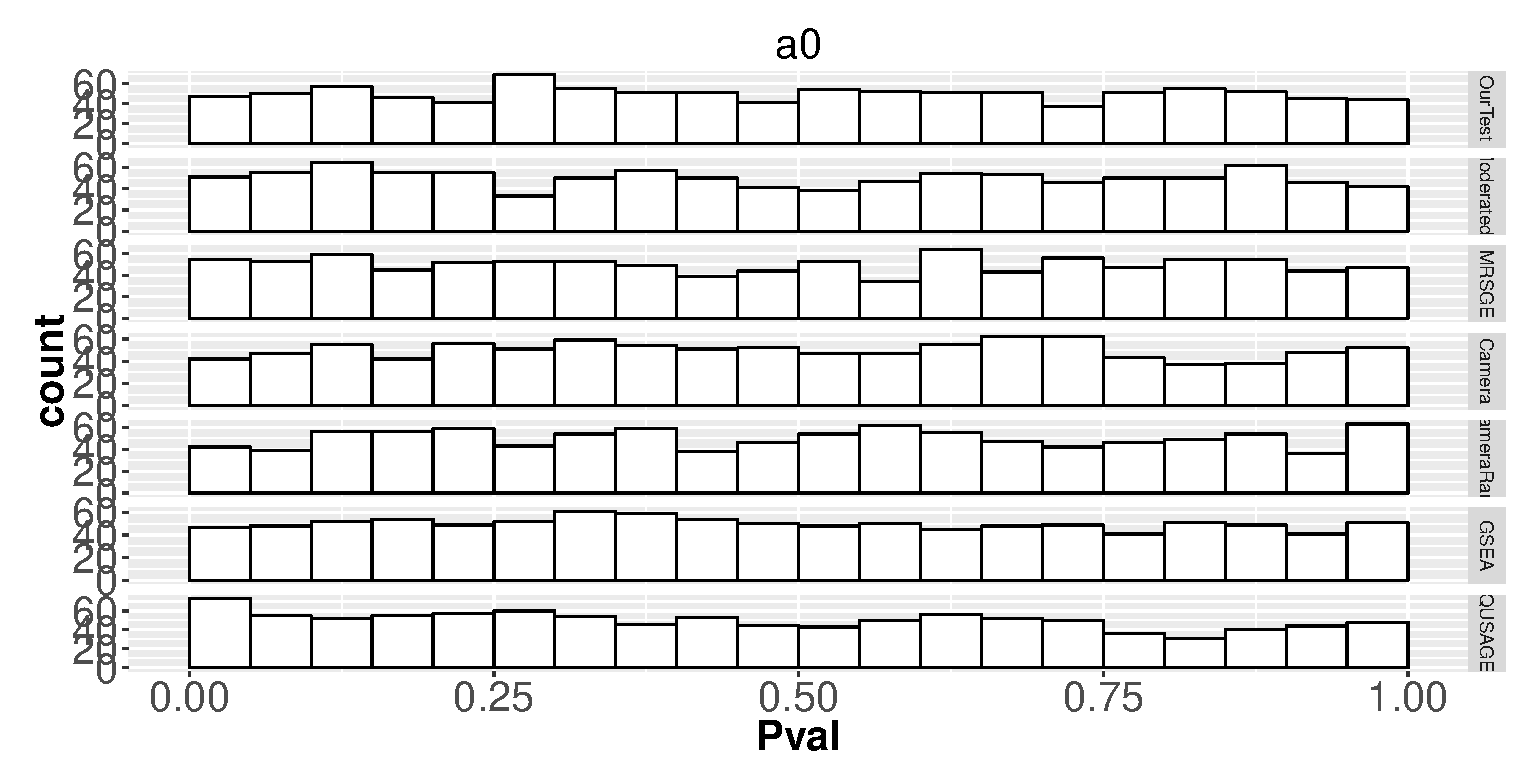
\includegraphics[width=8cm,height=5cm]{Figures/NODEA0.eps}
				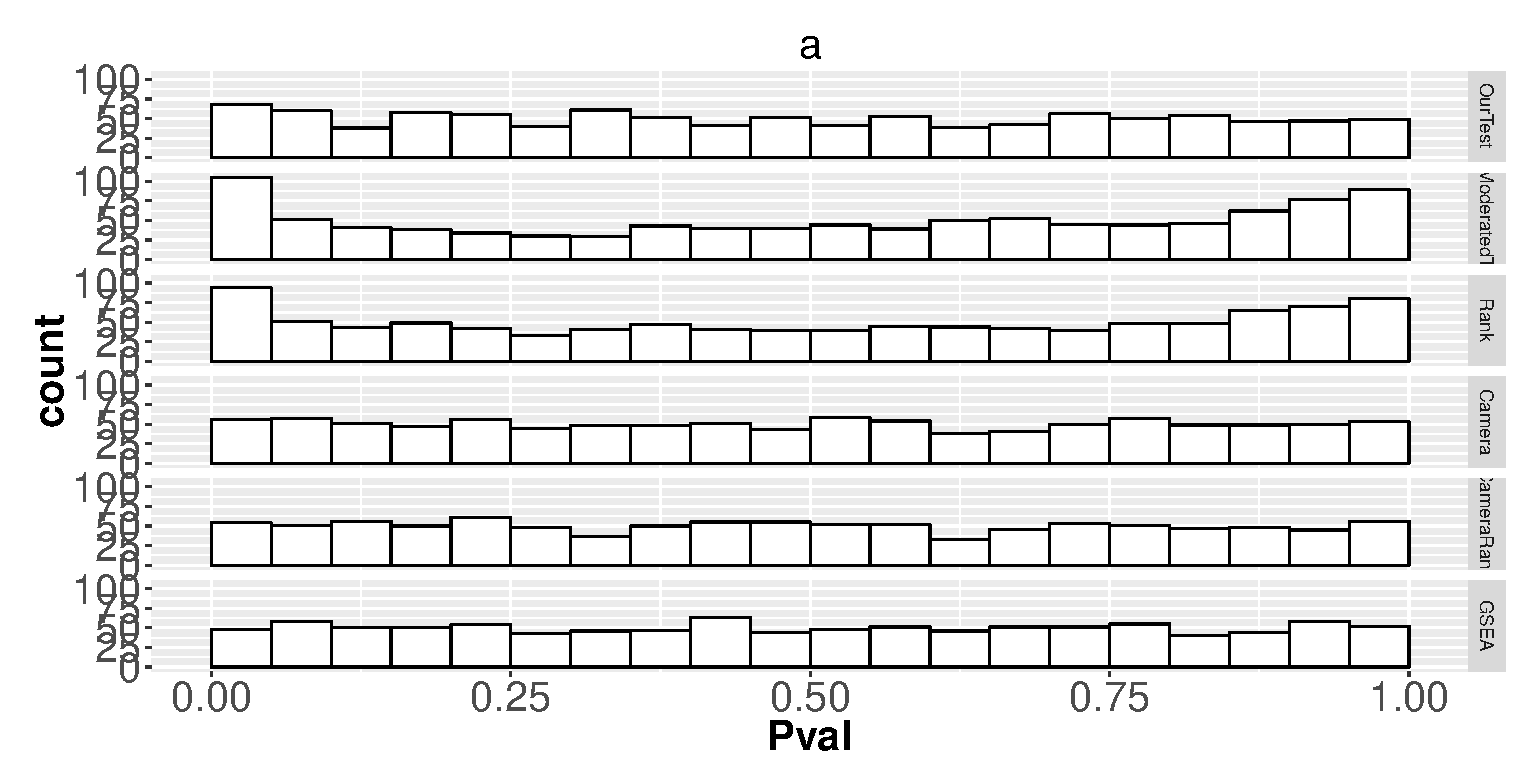
\includegraphics[width=8cm,height=5cm]{Figures/NODEA.eps}
				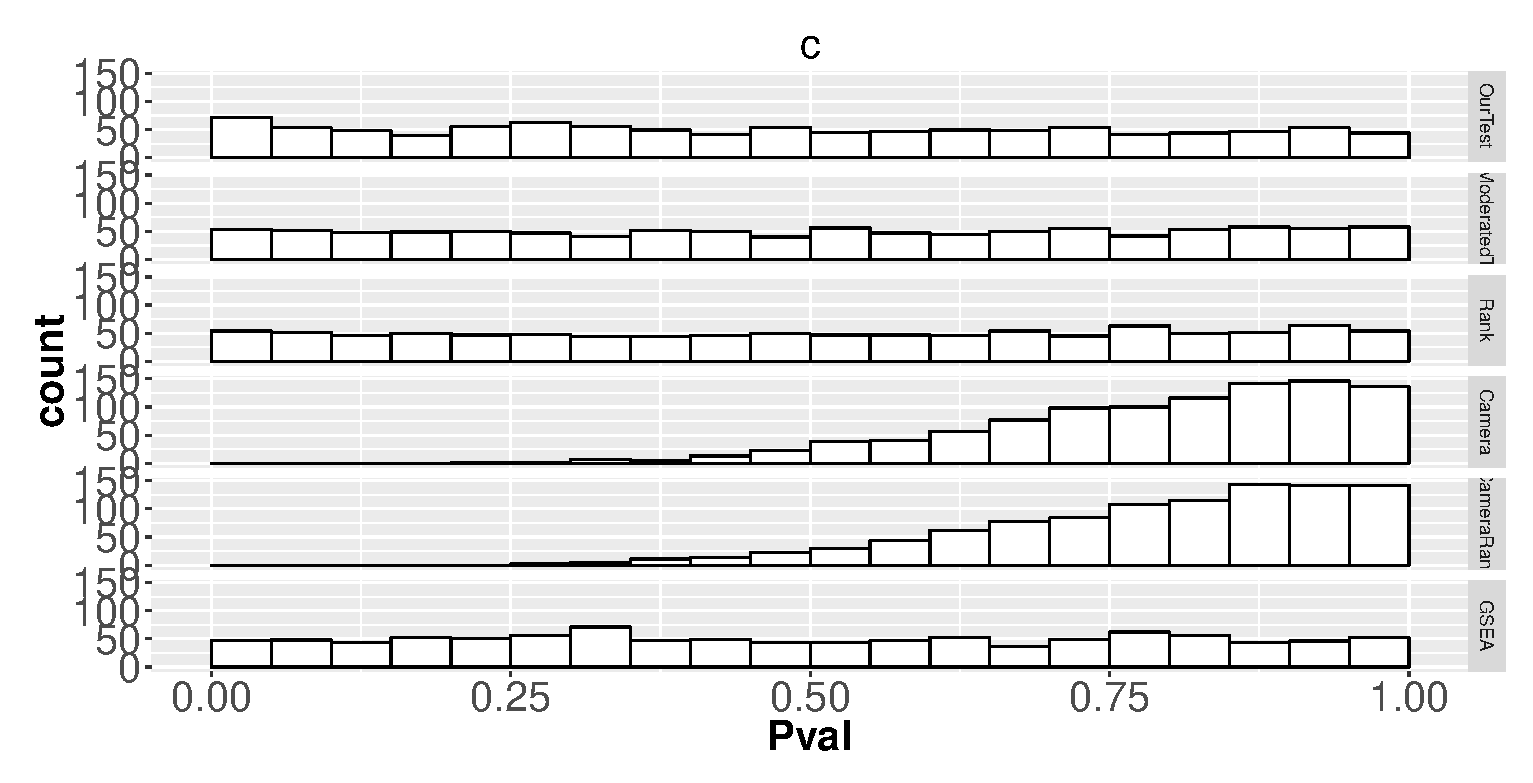
\includegraphics[width=8cm,height=5cm]{Figures/NODEC.eps}
				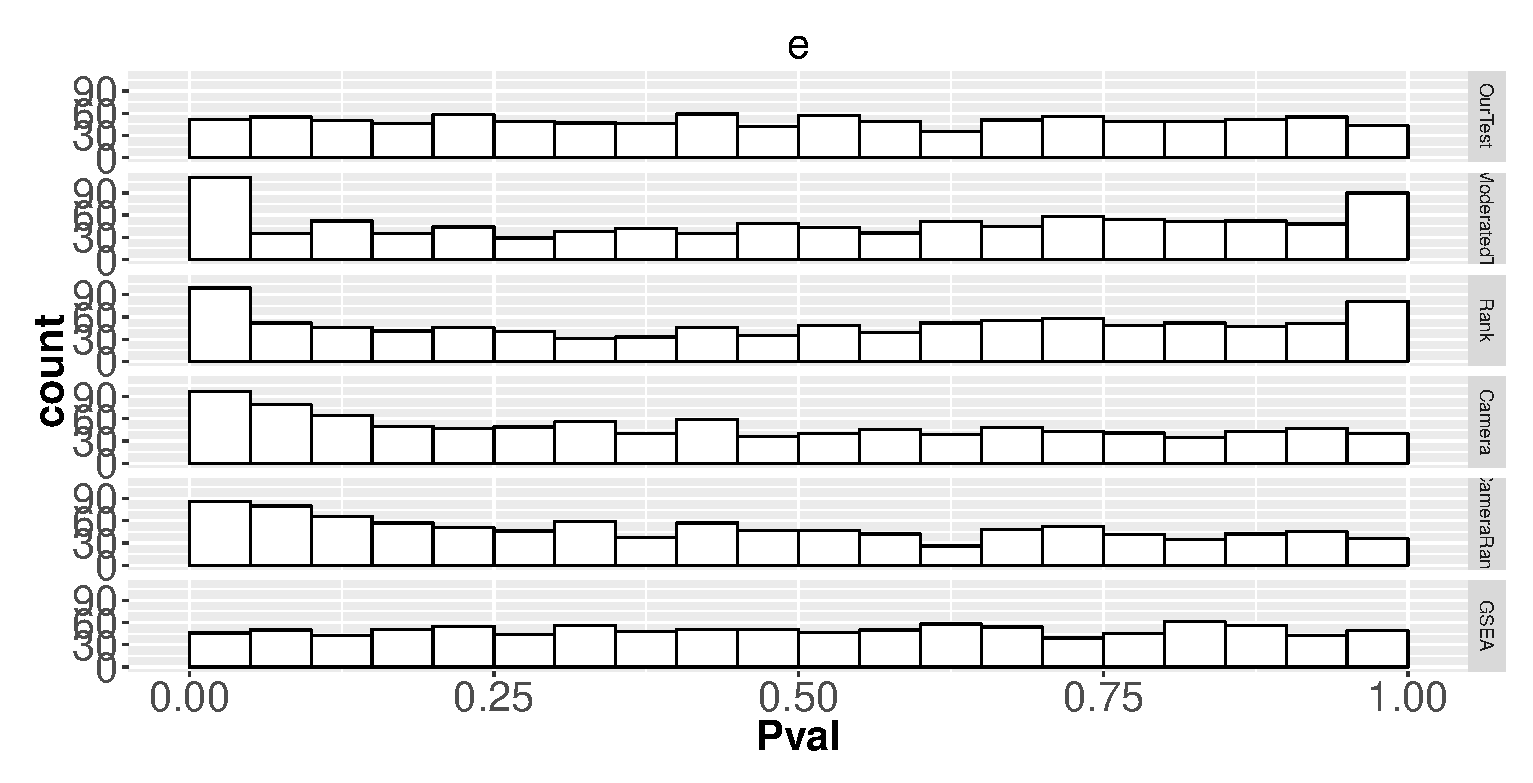
\includegraphics[width=8cm,height=5cm]{Figures/NODEE.eps}
				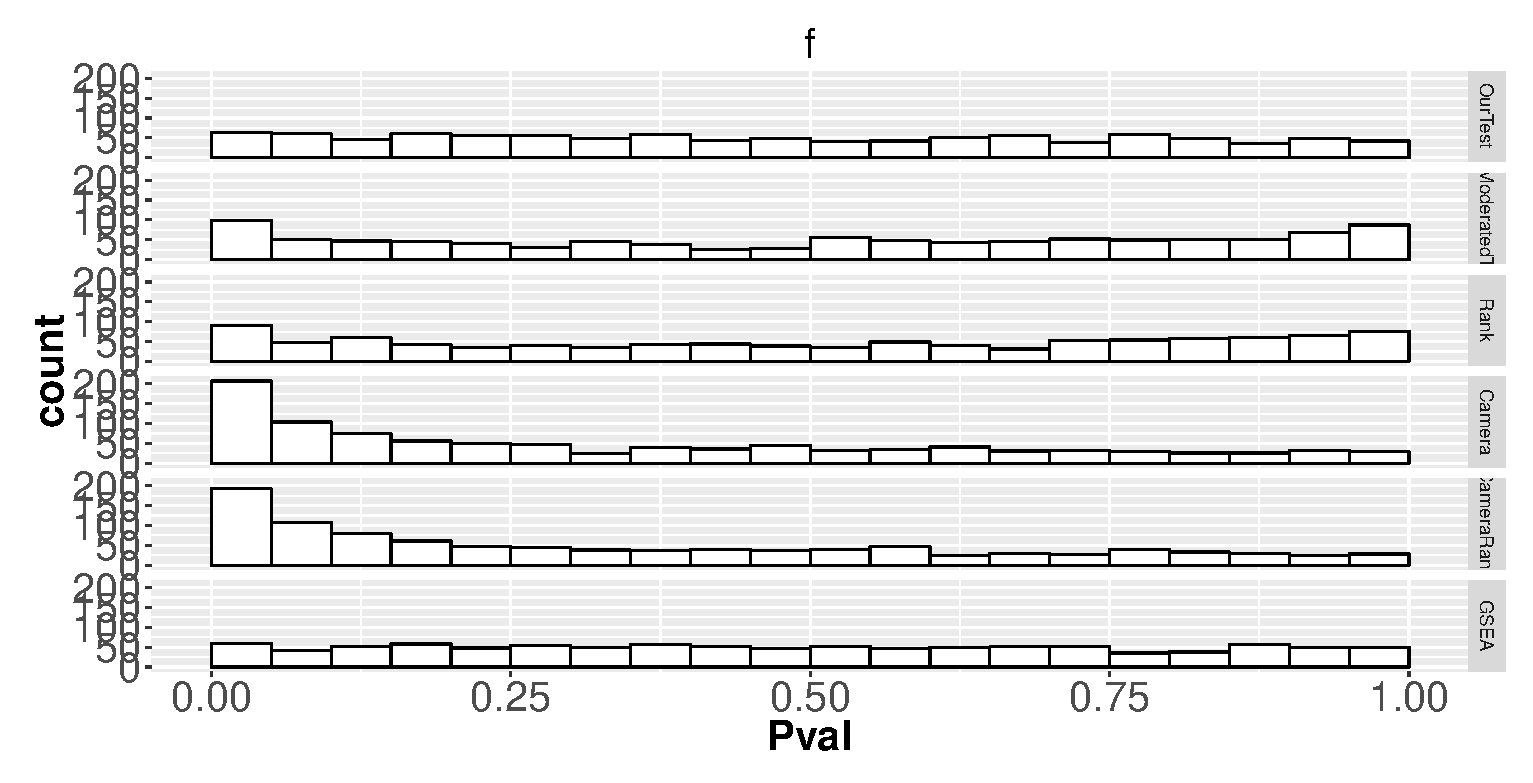
\includegraphics[width=8cm,height=5cm]{Figures/NODEF.eps}
				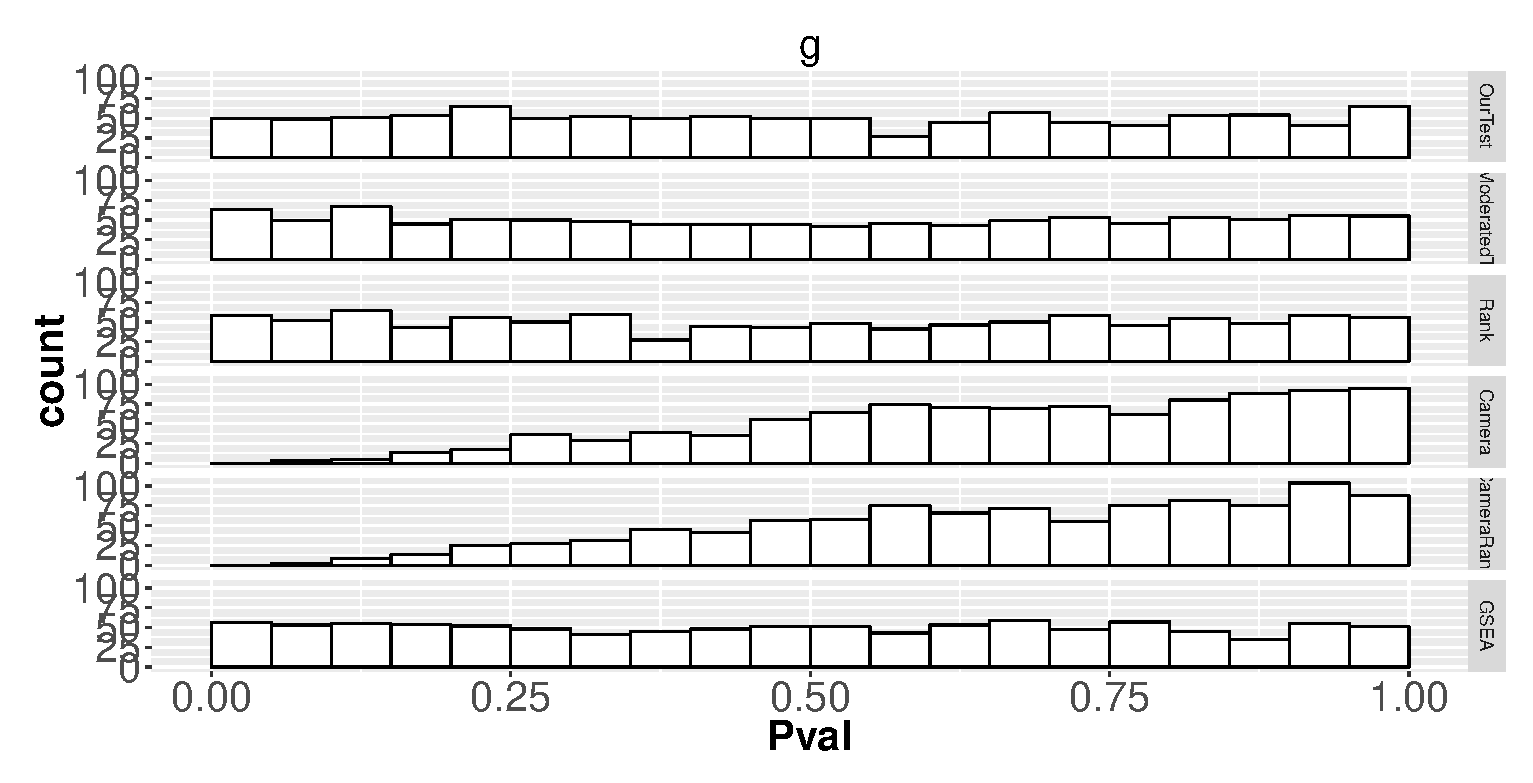
\includegraphics[width=8cm,height=5cm]{Figures/NODEG.eps}
			\end{center} 
		\end{figure} 
		
		
\begin{table}[ht]
	\centering
	\caption{Type I error rate of gene set tests for correlated expression values }\label{table:typeIerror}
	\begin{tabular}{lrrrrlrrrr}
		\hline
		\cline{1-10}
		\multicolumn{1}{l}{Method} &\multicolumn{4}{c}{Norminal $p$-values}&  & \multicolumn{4}{c}{Norminal $p$-values} \\ \cline{2-10} 
		 & 0.01 & 0.05 & 0.1 & 0.2 &    & 0.01 &0.05 & 0.1 & 0.2 \\ 
		\hline
		  & \multicolumn{4}{c}{(a0)} & & \multicolumn{4}{c}{(a)} \\
		OurTest & 0.012 & 0.066 & 0.124 & 0.241 &  & 0.011 & 0.049 & 0.097 & 0.198 \\ 
		geneSetTest-modt & 0.012 & 0.058 & 0.109 & 0.215 &  & 0.006 & 0.052 & 0.099 & 0.219 \\ 
		geneSetTest-rank & 0.012 & 0.055 & 0.110 & 0.214 &  & 0.018 & 0.060 & 0.116 & 0.202 \\ 
		CAMERA & 0.006 & 0.059 & 0.135 & 0.217 &  & 0.000 & 0.000 & 0.000 & 0.006 \\ 
		CAMERA-Rank & 0.003 & 0.054 & 0.112 & 0.229 &  & 0.001 & 0.009 & 0.023 & 0.079 \\ 
		GSEA & 0.989 & 0.995 & 0.997 & 0.997 &  & 0.228 & 0.608 & 0.794 & 0.927 \\ 
			 & \multicolumn{4}{c}{(c)} &  & \multicolumn{4}{c}{(e)} \\
		OurTest & 0.007 & 0.052 & 0.103 & 0.202 &  & 0.008 & 0.056 & 0.093 & 0.207 \\ 
		geneSetTest-modt & 0.007 & 0.051 & 0.098 & 0.187 &  & 0.015 & 0.058 & 0.106 & 0.217 \\ 
		geneSetTest-rank & 0.006 & 0.050 & 0.106 & 0.190 &  & 0.024 & 0.082 & 0.138 & 0.225 \\ 
		CAMERA & 0.000 & 0.000 & 0.000 & 0.000 &  & 0.000 & 0.000 & 0.001 & 0.009 \\ 
		CAMERA-Rank & 0.000 & 0.000 & 0.000 & 0.000 &  & 0.000 & 0.020 & 0.054 & 0.127 \\ 
		GSEA & 0.942 & 0.984 & 0.992 & 0.995 &  & 0.108 & 0.469 & 0.731 & 0.899 \\ 
			 & \multicolumn{4}{c}{(f)} & & \multicolumn{4}{c}{(g)} \\
		OurTest & 0.012 & 0.050 & 0.098 & 0.226 &  & 0.007 & 0.059 & 0.116 & 0.211 \\ 
		geneSetTest-modt & 0.010 & 0.071 & 0.115 & 0.213 &  & 0.010 & 0.061 & 0.104 & 0.218 \\ 
		geneSetTest-rank & 0.007 & 0.061 & 0.112 & 0.221 &  & 0.014 & 0.072 & 0.142 & 0.247 \\ 
		CAMERA & 0.000 & 0.000 & 0.004 & 0.019 &  & 0.000 & 0.000 & 0.001 & 0.006 \\ 
		CAMERA-Rank & 0.006 & 0.041 & 0.096 & 0.210 &  & 0.000 & 0.000 & 0.002 & 0.009 \\ 
		GSEA & 0.015 & 0.188 & 0.434 & 0.770 &  & 0.943 & 0.975 & 0.983 & 0.992 \\ 
		\hline
	\end{tabular}
\end{table}
		\subsubsection{Power simulation}
		WHAT TO PRESENT
		
		\subsection{Maybe real data analysis??? }
	\section{Conclusion}\label{section:conclusion}
	
	\section{AcknowledgeMents}\label{section:acknowledgement}
	
	\section{Appendix}\label{section:appendix}
	
	First $E(\Delta_i) = E(Z_i\delta_i) = E(Z_i)E(\delta_i) = p_i\mu_{\delta}$. Next note that  
	\[\text{Var}(\Delta_i) = E[(Z_i\delta_i)^2]- [E(Z_i\delta_i)]^2 = \text{Var}(Z_i)[E(\delta_i)]^2 + \left[(EZ_i)^2 + \text{Var}(Z_i)\right]\text{Var}(\delta_i) =p_i\sigma_{\delta}^2 + p_i(1-p_i)\mu_{\delta}^2\]
	
	Let $T_i=\bar{Y}_{i,2}-\bar{Y}_{i,1}$ be the difference in mean expression levels between the treatment group and the control group. We have 
	\[E(T_i) = E(\bar{Y}_{i,2})-E(\bar{Y}_{i,1}) = E(\Delta_i) = E(Z_i\delta_i) = p_i\mu_{\delta}\]
	The covariance between two genes $i_1$ and $i_2$ is given by (I HAVE CONCERNS HERE, IS IT VALID TO ASSUME THAT DE EFFECTS ARE INDEPENDENT BETWEEN GENES?  WE SEE CO-EXPRESSION!! OR WE'VE ALREADY TAKEN THAT INTO ACCOUNT BY "CORRELATION BETWEEN GENES"), 
	
				\begin{equation}
					\begin{aligned}
						\text{Cov}(T_{i_1}, T_{i_2}) & = E\left[\text{Cov}(T_{i_1}, T_{i_2}|\Delta_{i_1}, \Delta_{i_2}) \right]  + \text{Cov}\left[E(T_{i_1}|\Delta_{i_1}), E(T_{i_2}|\Delta_{i_2})\right] \\
						& = E\left(\frac{1}{n_1}\rho_{i_1,i_2} + \frac{1}{n_2}\rho_{i_1,i_2}\right) + \text{Cov}(\Delta_{i_1}, \Delta_{i_2})\\
						& = \left(\frac{1}{n_1} + \frac{1}{n_2}\right)\rho_{i_1,i_2}
					\end{aligned}
				\end{equation}
				For gene $i$, the variance $\text{Var}(T_i) = \text{Var}(\bar{Y}_{i, 1}) + \text{Var}(\bar{Y}_{i, 2})$, with
				\[\text{Var}(\bar{Y}_{i, 1}) = \frac{1}{n_1}\] 
				\begin{equation}
					\begin{aligned}
						\text{Var}(\bar{Y}_{i, 2}) & = \frac{1}{n_2^2}\left[\sum_{j=1}^{n_2}\text{Var}(Y_{ij2}) + 2\sum_{1\leq j_1<j_2 \leq n_2} \text{Cov}(Y_{ij_12}, Y_{ij_22})\right] \\
						& = \frac{1}{n_2}\text{Var}(Y_{ij2}) + \frac{n_2-1}{n_2} \text{Cov}(Y_{ij_12}, Y_{ij_22})\\
						& = \frac{1}{n_2}\left[E\left(\text{Var}(Y_{ij2}|\Delta_i)\right) + \text{Var}\left(E(Y_{ij2}|\Delta_i)\right)\right] \\ \text{~~~} &+\frac{n_2-1}{n_2}\left[E\left(\text{Cov}(Y_{ij_12}, Y_{ij_22}|\Delta_i)\right) + \text{Cov}\left(E(Y_{ij_12}|\Delta_i), E(Y_{ij_22}|\Delta_i)\right)\right] \\
						& = \frac{1}{n_2} + \text{Var}(\Delta_i)
					\end{aligned}
				\end{equation}
				Therefore $\text{Var}(T_i)  = \frac{1}{n_1} + \frac{1}{n_2} + \text{Var}(\Delta_i)$, and it follows 
				\begin{equation}\label{eq:tvar}
					\text{Cov}(\bm T) =  \bm D + \sigma_2^2\bm C 
				\end{equation}
				where $\bm D$ is a diagonal matrix with $\text{Var}(\Delta_i) =p_i\sigma_{\delta}^2 + p_i(1-p_i)\mu_{\delta}^2$ as its $i$th diagonal element, and $\sigma_2^2 = \left(\frac{1}{n_1} + \frac{1}{n_2}\right)$.

				
				
				
								
\newpage

\bibliographystyle{apalike}
\bibliography{mybib}
	
\end{document}
